\documentclass[11pt,a4paper]{article}
\usepackage[inline]{enumitem}
\usepackage{amsfonts}
\usepackage{amsmath,amssymb,amsthm}
\usepackage{mathtools}
\usepackage{graphicx, subcaption}
\usepackage[margin=1in,a4paper]{geometry}
\usepackage{algorithm}
\usepackage{algorithmic}
% \usepackage[font= scriptsize]{subcaption}
\usepackage{xcolor}
\usepackage{natbib}
\usepackage{tabu}
\usepackage{multirow} 
\usepackage[colorlinks,citecolor=blue,urlcolor=blue,bookmarks=false,hypertexnames=true]{hyperref} 
%\usepackage[utf8]{inputenc}
\usepackage{newunicodechar}
\providecommand{\keywords}[1]{\noindent\textbf{{Keywords:}} #1}
\usepackage{rotating}

\usepackage{mathtools}
\usepackage{setspace}
\mathtoolsset{showonlyrefs=true}
\newtheorem{proposition}{Proposition}
\newtheorem{corollary}{Corollary}
\newtheorem{lemma}{Lemma}
\newtheorem{definition}{Definition}
\newtheorem{assumption}{Assumption}
\newtheorem{theorem}{Theorem}
\theoremstyle{remark}
\newtheorem{remark}{Remark}
\newtheorem{example}{Example}
\setlength{\bibsep}{0.0pt}
\allowdisplaybreaks[4]

\usepackage{todonotes}

\title{Hamiltonian Neural Network for Pseudo Marginal Hamiltonian Monte Carlo}
\author{Yeda CUI}
\date{February 2, 2025}

\begin{document}

\maketitle

This report outlines my attempt to apply the Hamiltonian Neural Network (HNN) to the Pseudo Marginal HMC (PMHMC) method. Section \ref{sec:background} provides a recap of the PMHMC method introduced by \cite{alenlov2021pseudo}. Section \ref{sec:hnn} details my approach to developing an HNN-based method for PMHMC. Finally, Section \ref{sec:models} highlights financial models that can benefit from either HNN or PMHMC. All notations are consistent with those in \cite{alenlov2021pseudo}, unless otherwise specified.
\section{Background}
\label{sec:background}
\cite{alenlov2021pseudo} proposed PMHMC based on the extended Hamiltonian system defined in equation (10). Since the integration error increases with the dimensionality, they split the extended Hamiltonian $H$ into two components, $A$ and $B$, as follows: 
\begin{align}
	A(\rho, \mathbf{u}, \mathbf{p}):=\frac{1}{2}\left\{\rho^{\top} \rho+\mathbf{u}^{\top} \mathbf{u}+\mathbf{p}^{\top} \mathbf{p}\right\}, \quad B(\theta, \mathbf{u}):=-\log p(\theta)-\log \hat{p}\left(y_{1: T} \mid \theta, \mathbf{u}\right) ,
\end{align}
where both components have analytical solutions. The solutions of these two systems after $h$ units of time, denoted as $\Phi_h^A$ and $\Phi_h^B$, are as follows:
\begin{align}
	\Phi_h^A:\left\{\begin{array}{l}
\theta(h)=\theta(0)+h \rho(0) \\
\rho(h)=\rho(0) \\
\mathbf{u}(h)=\mathbf{p}(0) \sin (h)+\mathbf{u}(0) \cos (h) \\
\mathbf{p}(h)=\mathbf{p}(0) \cos (h)-\mathbf{u}(0) \sin (h)
\end{array}\right.
\end{align}
and
\begin{align}
\label{eq:phiB}
	\Phi_h^B:\left\{\begin{array}{l}
\theta(h)=\theta(0) \\
\rho(h)=\rho(0)+h \nabla_\theta\left\{\log p(\theta)+\log \hat{p}\left(y_{1 T T} \mid \theta, \mathbf{u}(0)\right)\right\}_{\mid \theta=\theta(0)} \\
\mathbf{u}(h)=\mathbf{u}(0) \\
\mathbf{p}(h)=\mathbf{p}(0)+h \nabla_{\mathbf{u}} \log \hat{p}\left(y_{1: T} \mid \theta(0), \mathbf{u}\right)_{\mid \mathbf{u}=\mathbf{u}(0)}
\end{array}\right. .
\end{align}
The numerical integration of the whole Hamiltonian system after $hL$ units of time is given by 
\begin{align}
	\hat{\Phi}_{h L}=\Phi_{h / 2}^A \circ\left\{\Phi_h^B \circ \Phi_h^A\right\}^{L-1} \circ \Phi_h^B \circ \Phi_{h / 2}^A.
\end{align}

\smallskip
\noindent \textbf{Sampling under Generalized Linear Mixed Model} I implemented the PMHMC method introduced in \cite{alenlov2021pseudo}. While replicating the results from Section 4.3 and using the same prior and initial marginal state $\theta$, my sampled values for $\mu_1$ and $\mu_2$ did not concentrate in the correct region. To address this, I adopted a narrower prior, specifically $N(0,1)$, for all $\theta$. Additionally, the initial states for $\log \lambda_1$, $\log \lambda_2$, and $\text{logit}\, w_1$ were set to zero. Under these modified settings, the sampling results appeared much more reasonable, as illustrated in Figure \ref{fig:pmhmcplots}.

\begin{figure}
\centering
	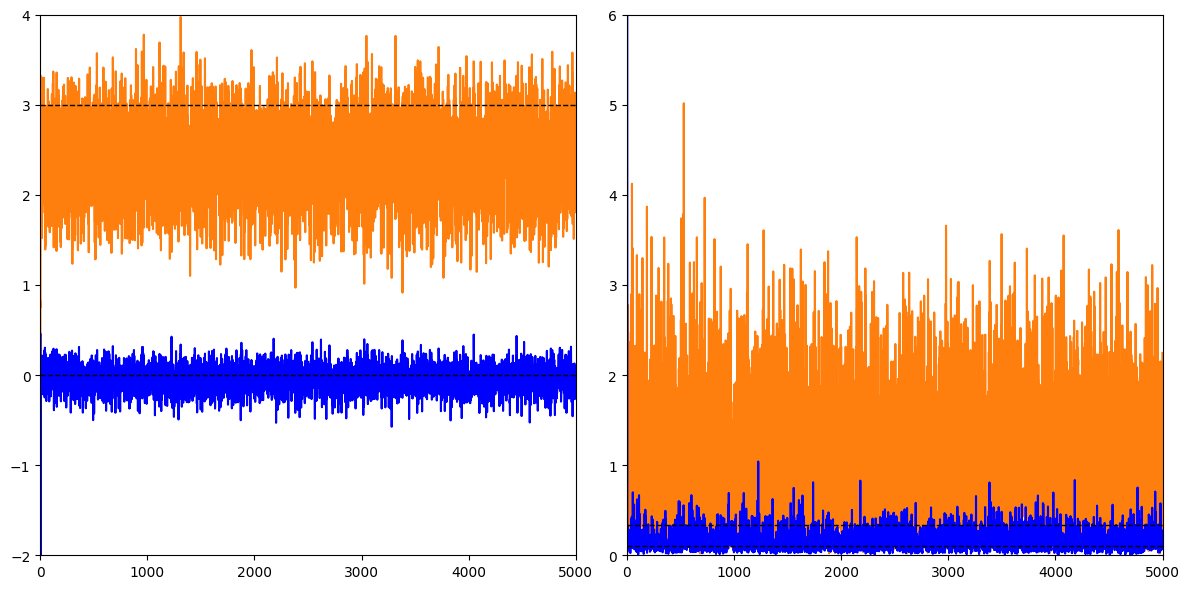
\includegraphics[width=0.6\textwidth]{../figures/pmhmcplots.png}
	\caption{Traces for parameters $\mu_1$ and $\mu_2$ (left) and $1/\lambda_1$ and $1/\lambda_2$ (right) for the pseudo-marginal HMC sampler with N = 128.}
	\label{fig:pmhmcplots}
\end{figure}


\section{Hamiltonian Neural Network for PMHMC}
\label{sec:hnn}
Based on my understanding, since the Hamiltonian system A is explicit and has an analytical solution, it's only necessary to use an HNN to learn the Hamiltonian system B and replace the numerical partial derivatives in Equation \eqref{eq:phiB}.  For some network paramters $\phi$, let $H_\phi(\theta, \rho, \mathbf{u}, \mathbf{p})$ represents the HNN's prediction of the Hamiltonian system B. To train the HNN, we can adopt the same loss function proposed in \cite{greydanus2019hamiltonian} and \cite{dhulipala2023efficient}. Given training data $\{\theta, \rho, \mathbf{u}, \mathbf{p}\}$, numerical gradients are first computed to give the numerical time derivatives $\left\{\frac{d \theta}{d t}, \frac{d \rho}{d t}, \frac{d \mathbf{u}}{d t}, \frac{d \mathbf{p}}{d t}\right\}$ as follows:
\begin{align}
	&\frac{d \theta}{d t} = 0, \quad \frac{d \rho}{d t} =  \nabla_\theta\left\{\log p(\theta)+\log \hat{p}\left(y_{1 T T} \mid \theta, \mathbf{u}(0)\right)\right\}_{\mid \theta=\theta(0)} ,\\
	&\frac{d \mathbf{u}}{d t} = 0, \quad \frac{d \mathbf{p}}{d t} = \nabla_{\mathbf{u}} \log \hat{p}\left(y_{1: T} \mid \theta(0), \mathbf{u}\right)_{\mid \mathbf{u}=\mathbf{u}(0)}.
\end{align}
HNNs optimize the network parameters $\phi$ to minimize the following loss function:
\begin{align}
	L=\left\|\frac{\partial H_\phi}{\partial \rho}-\frac{d \theta}{d t}\right\|+\left\|-\frac{\partial H_\phi}{\partial \theta}-\frac{d \rho}{d t}\right\| + \left\|\frac{\partial H_\phi}{\partial \mathbf{p}}-\frac{d \mathbf{u}}{d t}\right\|+\left\|-\frac{\partial H_\phi}{\partial \mathbf{u}}-\frac{d \mathbf{p}}{d t}\right\|.
\end{align}
After training the neural network, the integration solution for the Hamiltonian system $B$ can be approximated as:
\begin{align}
\label{eq:phiBapprox}
	\tilde{\Phi}_h^B:\left\{\begin{array}{l}
\theta(h)=\theta(0) \\
\rho(h)=\rho(0) - h \frac{\partial H_\phi}{\partial \theta} (\theta (0), \rho(0), \mathbf{u}(0), \mathbf{p}(0))\\
\mathbf{u}(h)=\mathbf{u}(0) \\
\mathbf{p}(h)=\mathbf{p}(0)- h \frac{\partial H_{\phi}}{\partial \mathbf{p}} (\theta (0), \rho(0), \mathbf{u}(0), \mathbf{p}(0))
\end{array}\right. .
\end{align}
The numerical integration of the whole Hamiltonian system after $hL$ units of time can be approximated by 
\begin{align}
\label{eq:integratorapprox}
	\tilde{\Phi}_{h L}=\Phi_{h / 2}^A \circ\left\{\tilde{\Phi}_h^B \circ \Phi_h^A\right\}^{L-1} \circ \tilde{\Phi}_h^B \circ \Phi_{h / 2}^A.
\end{align}


\subsection{PMHMC by L-HNN in \cite{dhulipala2023efficient}}
Firstly, I attempted to directly adopt the L-HNN structure proposed in \cite{dhulipala2023efficient}, where $H_\phi$ is represented as a feedforward neural network. The input dimension of the network is $2d + 2D$. For the generalized linear mixed model example discussed in Section 4.3 of \cite{alenlov2021pseudo}, $d = 13$ and $D = 64,000$, resulting in a neural network input dimension of $128,026$ which is dramatically higher than the examples in \cite{dhulipala2023efficient}, where the highest input dimension is only $100$. Both the input and output dimensions in the training dataset are also high-dimensional. 

Unlike \cite{dhulipala2023efficient}, where the entire dataset can be loaded into memory for training, this is not feasible here due to memory limitations. Instead, I loaded batches of data into memory for training and utilized the TFRecord data format to improve I/O efficiency, as opposed to the pickle format used in \cite{dhulipala2023efficient}. For training, I used a batch size of 512, a learning rate of 0.001, and 10,000 training steps. However, the training mean squared error loss only decreased to 0.01. Figure \ref{fig:lhnn} compares the gradient of the Hamiltonian with respect to the marginal variables $\theta$, computed via autograd and the predictions of the HNN. Figure \ref{fig:lhnngrads} shows that the partial derivatives computed by the LHNN are significantly incorrect. Additionally, Figure \ref{fig:hamildiff} demonstrates that the Hamiltonian cannot be conserved during integration using Equation \eqref{eq:integratorapprox}. The acceptance rate using LHNNs is nearly zero. I also tested different learning rates $\{0.1,0.01,0.0001\}$ and neural network widths $500, 2000$, but the results remained similar.
\begin{figure}[h!]
\centering
\subcaptionbox{\label{fig:lhnngrads}}{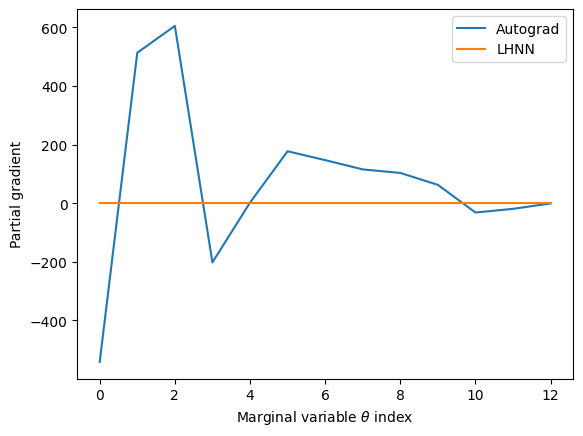
\includegraphics[width=0.3\textwidth]{../figures/lhnngrads.png}}
\quad
\subcaptionbox{\label{fig:hamildiff}}{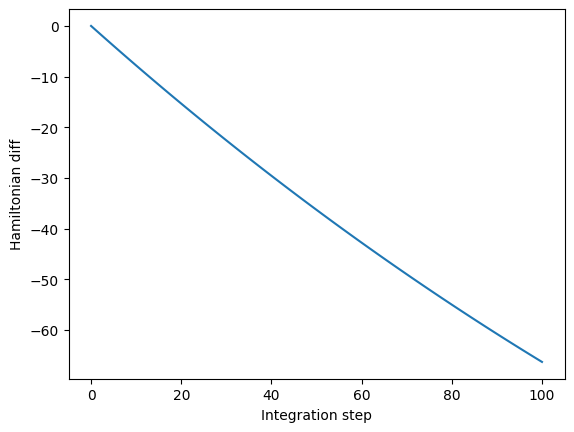
\includegraphics[width=0.3\textwidth]{../figures/hamildiff.png}}
\caption{(a) The partial derivatives of the 13 marginal parameters computed by autograd and LHNN. 
(b) The Hamiltonian path after 100 steps of integration using LHNN via Equation~\eqref{eq:integratorapprox}.}
\label{fig:lhnn}
\end{figure}

To investigate why the loss cannot be further reduced, I speculate that the issue arises from the high dimensionality of the problem, which limits the LHNN's ability to effectively represent the Hamiltonian system. To test this hypothesis, I used the LHNN to learn the Hamiltonian of standard normal density for a total of only $16$ samples under varying dimensions. The setup involved a three-layer neural network with a width of $500$, trained over $100$ epochs, with $1000$ training steps per epoch. The mean squared error (MSE) loss paths during training are shown in Figure \ref{fig:losscmp}. From this figure, we observe that when the dimension is as high as $25,000$, the LHNN struggles to train effectively and fails to learn the Hamiltonian gradients of the $16$ standard normal samples. This suggests that the learning capacity of the LHNN under high dimensions is limited. It is important to note that this test involves a relatively simple task---learning the gradients of the Hamiltonian for only $16$ samples drawn from a standard normal distribution. For more complex tasks, such as learning the Hamiltonian for the general linear mixed model, more sophisticated architectures are likely required. 

\smallskip
\noindent \textbf{Advantage with HNN} One advantage of the HNN approach is that the simulation process is significantly faster. For example, in the generalized linear mixed model discussed in Section 4.3 of \cite{alenlov2021pseudo}, there are a total of $3000$ observations, making the calculation of gradients for the Hamiltonian system highly time-consuming. In contrast, computing the gradient using the HNN is considerably more efficient.


\begin{figure}
\centering
	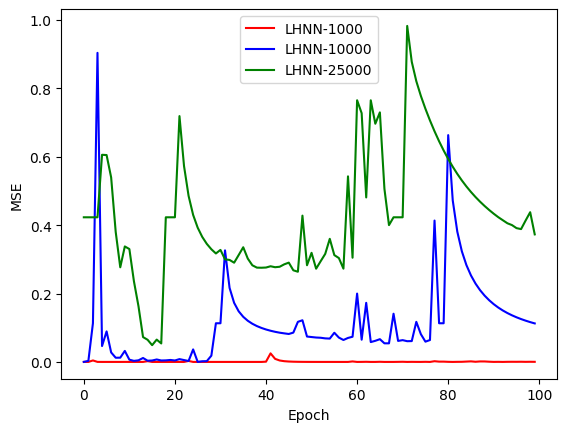
\includegraphics[width=0.3\textwidth]{../figures/losscmp.png}
	\caption{The MSE loss path for learning the Hamiltonian gradients of standard normal density with varying dimensions.}
	\label{fig:losscmp}
\end{figure}


\subsection{Modifications to the Structure of HNN for PMHMC} 
Due to the high dimensionality of the problem, I proposed a modification to the structure of the HNN to reduce the input dimension of the neural network. It is observed that the Hamiltonian $B$ can be expressed as the summation of simple functions with different inputs:
\begin{align}
    B = -\log p(\theta) - \log \hat{p}(y_{1:T} \mid \theta, \mathbf{U}) = -\log p(\theta) - \sum_{k=1}^T \log \hat{p}(y_k \mid \theta, \mathbf{U}_k).
\end{align}
We can utilize a neural network $\mathcal{H}_\phi (y, \theta, u)$ to approximate the function $-\log \hat{p}(y \mid \theta, u)$. The HNN for predicting $B$ is then defined as:
\[
H_\phi (\theta, \rho, \mathbf{u}, \mathbf{p}) = \frac{1}{2} \theta^T \theta + \sum_{k=1}^T \mathcal{H}_\phi (y_k, \theta, \mathbf{u}_k),
\]
where the prior of $\theta$ is assumed to be a normal distribution. I implemented this idea; however, the results are still unsatisfactory and the acceptance rate is still close to zero.


\section{Beneficial Financial Models by \cite{alenlov2021pseudo} or \cite{dhulipala2023efficient}}
\label{sec:models}
\smallskip
\noindent \textbf{Stochastic Volatility Model} 

The stochastic volatility (SV) model is a widely used framework in financial econometrics for modeling time-varying volatility in financial time series. It assumes that the observed series is driven by a latent (unobservable) volatility process that evolves stochastically over time. The general form of the SV model is given by:
\begin{align}
    dS_t &= \mu S_t \, dt + \sqrt{\nu_t} S_t \, dW_t, \\
    d\nu_t &= \alpha_{\nu,t} \, dt + \beta_{\nu,t} \, dB_t,
\end{align}
where $S_t$ is the stock price process and $\nu_t$ is the volatility process. While $S_t$ can be observed, $\nu_t$ is latent and unobservable. If we perform posterior estimation of both the model parameters and $\nu_t$, several challenges arise: The Metropolis-Hastings algorithm faces difficulties in selecting a proper proposal density for the latent volatility process $\nu_t$. The traditional HMC method struggles when the posterior distribution of $\nu_t$ exhibits strong multimodality. For example, the posterior distribution of $\nu_t$ under the Heston model shows strong multimodes, as shown in Section 2.3 of \cite{cape2015estimating}. The PMHMC method can overcome the multimodality issue, making it a suitable approach for such problems.
\begin{remark}
	Similarly, the posterior of the latent regime variable in regime-switching models also exhibits multimodality issues, making it a good candidate for benefiting from PMHMC. Other models with some variables that exhibit multimodality, but where we are not concerned with their distribution, can also leverage PMHMC effectively.
\end{remark}

\smallskip
\noindent \textbf{Credit Risk Modeling with Large Loan Portfolios} 
Credit risk modeling is crucial for financial institutions to estimate the probability that borrowers will default on their loan obligations. In the logistic regression model, the probability of default for borrower $i$ is modeled as:
\begin{align}
	P(Y_i = 1 \mid \mathbf{X}_i) = \frac{1}{1 + e^{-(\beta_0 + \mathbf{X}_i^\top \boldsymbol{\beta})}},
\end{align}
where $Y_i$ is a binary variable indicating default ($Y_i = 1$) or non-default ($Y_i = 0$), $\mathbf{X}_i$ is a vector of predictor variables for borrower $i$, and $\boldsymbol{\beta}$ is a vector of coefficients corresponding to the predictor variables.

Although $\boldsymbol{\beta}$ can be estimated using regression techniques, obtaining the posterior distribution of $\boldsymbol{\beta}$ is often desirable. The posterior distribution allows for the incorporation of prior information and enables robust risk analysis, such as assessing tail risk or calculating Conditional Value-at-Risk (CVaR) based on $\boldsymbol{\beta}$.

When dealing with large datasets, such as loan portfolios with a vast number of observations, traditional HMC methods can become computationally expensive and inefficient. This is due to the high cost of computing gradients for the entire dataset during each sampling iteration. However, the HNN approach introduced in \cite{dhulipala2023efficient} provides a significantly more efficient method for sampling from the posterior distribution. The HNN framework leverages second-order information, allowing for faster convergence and improved computational efficiency, making it suitable for large-scale credit risk modeling.

\begin{remark}
	Similarly, other models with a large number of observations, where traditional HMC becomes computationally expensive, can also benefit from the efficient sampling capabilities of HNN.
\end{remark}

\begin{remark}[Testing]
	All the source code is located in the ./src/ folder, with each Python script having a corresponding test file in the ./tests/ folder to validate all the classes and functions.
\end{remark}

\bibliographystyle{chicagoa}
\bibliography{refs}

\end{document}